\uuid{Ta23}
\exo7id{5820}
\auteur{rouget}
\organisation{exo7}
\datecreate{2010-10-16}
\isIndication{false}
\isCorrection{true}
\chapitre{Conique}
\sousChapitre{Ellipse}

\contenu{
\texte{
$(\mathcal{C})$ est le cercle de diamètre $[AB]$. $(\mathcal{D})$ est la tangente en $A$ au cercle $(\mathcal{C})$. $P$ est un point variable sur le cercle $(\mathcal{C})$ et $(\mathcal{T})$ la tangente en $P$ au cercle $(\mathcal{C})$. $(\mathcal{T})$ recoupe $(\mathcal{D})$ en $S$. La perpendiculaire à la droite $(AB)$ passant par $P$ coupe la droite $(BS)$ en $M$. Ensemble des points $M$ ?
}
\reponse{
On choisit un repère orthonormé $\mathcal{R}$ dans lequel le point $A$ a pour coordonnées $(1,0)$ et le point $B$ a pour coordonnées $(-1,0)$. Dans le repère $\mathcal{R}$, la droite $(\mathcal{D})$ a pour équation $x = 1$. Ensuite, il existe un réel $\theta$ tel que le point $P$ ait pour coordonnées $(\cos\theta,\sin\theta)$. La tangente $(\mathcal{T})$ a pour équation $x\cos\theta + y\sin\theta = 1$. Pour $\theta\notin\pi\Zz$, le point $S$ a pour coordonnées $\left(1,\frac{1-\cos\theta}{\sin\theta}\right)$ ou encore $\left(1,\tan\left(\frac{\theta}{2}\right)\right)$.

$$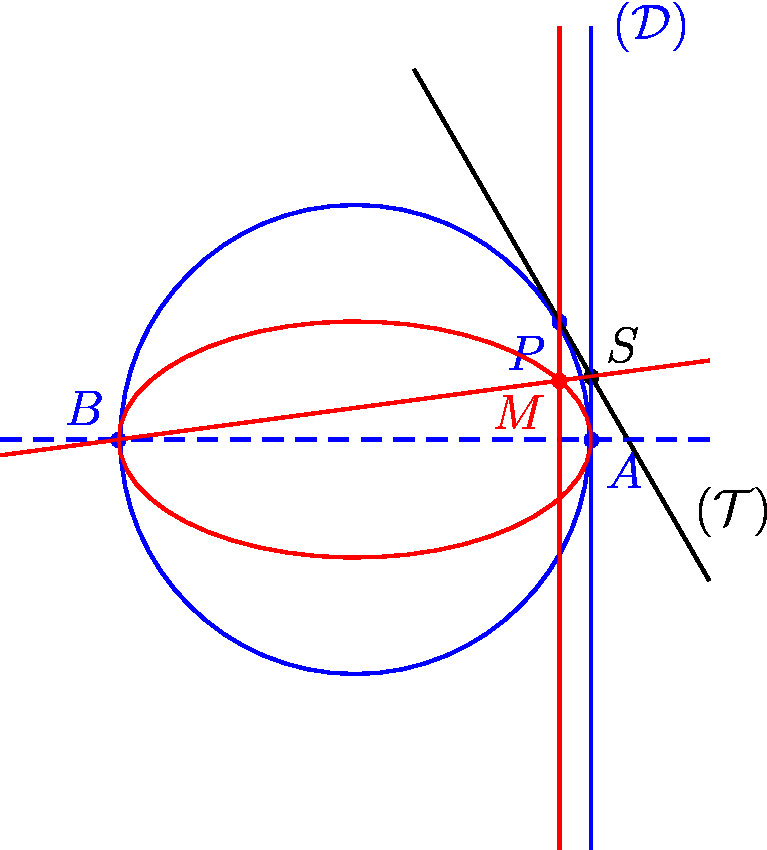
\includegraphics{../images/img005820-1}$$


La perpendiculaire à la droite $(AB)$ passant $P$ admet pour équation $x=\cos\theta$. La droite $(BS)$ admet pour équation $-\tan\left(\frac{\theta}{2}\right)(x+1)+2y=0$. Ces deux droites se coupent en le point $M$ de coordonnées $\left(\cos\theta,\frac{1}{2}\tan\left(\frac{\theta}{2}\right)(1+\cos\theta)\right)$ ou encore $\left(\cos\theta,\cos\left(\frac{\theta}{2}\right)\sin\left(\frac{\theta}{2}\right)\right)$ ou enfin $(\cos\theta,\frac{1}{2}\sin\theta)$.

L'ensemble des points $M$ est donc l'ensemble des points de coordonnées $\left(\cos\theta,\frac{1}{2}\sin\theta\right)$ quand $\theta$ décrit $\Rr\setminus\pi\Zz$ ou encore l'ellipse d'équation $x^2+4y^2 = 1$ privée des points $A$ et $B$.
}
}
